
\chapter {Haptics rendering algorithms}
In HAPI a haptics rendering algorithm (or haptics renderer) is a class
responsible for determining the forces and torque to render depending
on position and other data from the haptics device and all the shapes
the user has added to the scene. 

\section{Proxy based rendering}
All the algorithms supported by HAPI (both internally implemented and
external libraries such as OpenHaptics and Chai3D) use some variant of
proxy based haptics rendering. The proxy based rendering technique
involves having a virtual representation of the haptics device called
the proxy. The proxy follows the position of the haptics device, but
is not allowed to penetrate any surface. This means that when a
geometry is touched the proxy stays on the surface of the object, even
if the haptics device actually has penetrated the surface. Forces are
then generated to bring the haptics device out of the surface, towards
the proxy, and usally some kind of spring force between the proxy and
haptics device is used. When the user moves the haptics device inside
the object the proxy follows the movement, but on the surface. How the
surface follows determines how the structure of the surface will
feel. For example, if the proxy is always moved to a local minimum on
the distance to the surface, the surface will feel completely smooth,
but if the proxy is dragging behind you can get friction effects. In
HAPI the user can control both the forces generated and the movement
of the proxy.

\begin{figure} 
  \centering 
  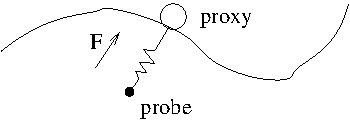
\includegraphics{images/proxyfinger.pdf}
  \caption{The proxy stays on the surface when the haptics
  device (probe) penetrates the surface. The resulting force is most
  commonly a spring force pushing the probe back towards the proxy.} 
  \label{Proxy-probe} 
\end{figure}



In the algorithms in HAPI the geometry of the proxy is either a point
or a sphere. The problem with point proxies is that it can fall
through small gaps in the geometry and makes it very hard to be able
to touch small, thin objects. Sphere problems... 

\section{Available algorithms}
There are four algorithms available in HAPI, where two are internally
implemented and two uses external haptics libraries. We will list them
and point out their uses, advantages/disadvantages etc.

\subsection{God-Object algorithm}
The god-object algorithm is based on the God-object paper( reference)
by .... It uses a point proxy .
- Point proxy
- User defined surfaces

\subsection{Ruspini algorithm}
The ruspini renderer is based on the algorithm presented by Ruspini in
(reference). It uses a sphere proxy.
- Sphere proxy
- User defined surfaces


\subsection{Chai3D}
- Sphere proxy(but not good)
- No user defined surfaces
- No magnetic surfaces

\subsection{OpenHaptics}
- Point based
- Only devices from SensAble
- No user defined surfaces

\section{Surfaces}
(TODO)
The way to specify how an object should feel in HAPI is done by
specifying an instance of a HAPISurfaceObject class that implements
the behavior. See ref specifying geometres. There are a couple of
surfaces already available in HAPI. They are:

(TODO Change to FrictionSurface!! take away bumpMap??)
\begin{itemize}
\item SmoothSurface - A SmoothSurface is a frictionless surface, where
  the proxy is always moved to minimize the distance between proxy and
  probe position. 
\item FrictionalSurface - Has additional parameters for specifying
  static and dynamic friction.
\item MagneticSurface - Surface pulls the haptics device towards the
  surface when within a user specified distance.
\item BumpmapSurface - Use a texture to define the height 
\item StiffnessFunctionSurface - Use a generic function to generate
  the normal force. The function takes the penetration depth as input
  and returns the corresponding force. 
\end{itemize}

There are also some surfaces specific for the OpenHaptics and Chai3D
libraries which allows the user to set the parameters available in
those libraries directly. They are:
\begin{itemize}
\item OpenHapticsSurface - Has all the parameters available in
  MagneticSurface, i.e. stiffness, staticFriction, etc, but instead of
  specifying them in the HAPI way in absolute units, they are all
  specified as a value between 0 and 1. A value of 0 for the stiffness
  means no stiffness at all and a value of 1 means the maximum
  stiffness the device can handle.
\item Chai3DSurface?? Don't know yet if it has any special parameters.
\end{itemize}

\subsection{User defined surfaces}

\begin{figure} 
  \centering 
  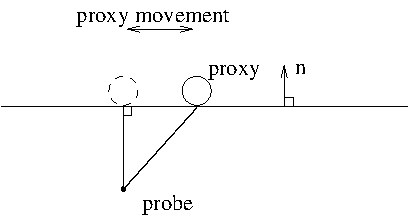
\includegraphics{images/surface.pdf}
  \caption{The flow of execution in the haptics thread.}
  \label{haptics thread} 
\end{figure}

Surfaces can be created for arbitrary force functions and proxy
movements. This is done by subclassing the HAPISurfaceObject class and
implementing the onContact() method. The purpose of the onContact
function is for the user to specify force and wanted proxy
movement. To understand the argument given to the onContact function
we will have to go through some preliminaries. When in contact with
the surface there will be a local surface approximation at the contact
point in the form of a plane. The argument given to the onContact
function is a ContactInfo structure. It contains information of the
contact and is also the structure used for returning force and proxy
movement. The input to the user is:


\begin{itemize}
\item Contact point(proxy position)
\item Probe position
\item Texture coordinate
\item Proxy radius
\item Shape id
\end{itemize}

All positions can be obtained in either global coordinates system or
in a local coordinate system with the plane normal as the y-axis and
contact point as the origin and two arbitrary perpendicular axis in
the plane as x and z-axis. This means that the penetration depth is
the same as -y in the local coordinate system. There are also function
available for converting between the global and local coordinate
system.

\begin{itemize}
\item Force
\item Torque
\item Proxy movement
\item Force position jacobian
\item Force velocity jacobian

\end{itemize}

.
.
.

